% This version of CVPR template is provided by Ming-Ming Cheng.
% Please leave an issue if you found a bug:
% https://github.com/MCG-NKU/CVPR_Template.

%\documentclass[review]{cvpr}
\documentclass[final]{cvpr}
\usepackage[OT1]{fontenc} 
\usepackage{times}
\usepackage{epsfig}
\usepackage{graphicx}
\usepackage{amsmath}
\usepackage{amssymb}
\usepackage{subfigure} 
\usepackage{float}
\usepackage{multicol}
\usepackage{stfloats}
\usepackage[toc,page]{appendix}
% Include other packages here, before hyperref.

% If you comment hyperref and then uncomment it, you should delete
% egpaper.aux before re-running latex.  (Or just hit 'q' on the first latex
% run, let it finish, and you should be clear).
\usepackage[pagebackref=true,breaklinks=true,colorlinks,bookmarks=false]{hyperref}
\usepackage{cleveref}
\def\cvprPaperID{****} % *** Enter the CVPR Paper ID here
\def\confYear{CVPR 2021}
%\setcounter{page}{4321} % For final version only


\begin{document}

%%%%%%%%% TITLE
\title{Report of Assignment 2}

\author{Xiangjian Hou*, Ning Sun*, Yufei Zhang*\\
Mohamed bin Zayed University of Artificial Intelligence\\
{\tt\small \{xiangjian.hou, ning.sun, yufei.zhang\}@mbzuai.ac.ae}
}

\maketitle

%%%%%%%%% ABSTRACT

%%%%%%%%% BODY TEXT

%-------------------------------------------------------------------------
\section{Introduction}
Image processing methods based on deep learning have made a lot of achievements, but traditional image processing methods still have irreplaceable advantages.

We compare the advantages and disadvantages of two different methods in edge detection, and the necessity of normalization is verified by experiments in blob detection. We try group of hyper-parameters to find the best result which gives in the \hyperref[append]{Appendices}.


%------------------------------------------------------------------------
\section{Implementation Details}

In this section, we introduce the principles of the algorithm used in the assignment.
\subsection{Canny Edge Detection}
We discuss about three main tools that need to be used for the canny edge detection.


%-------------------------------------------------------------------------
\subsubsection{Gaussian \& Sobel Mask}

The 2D Gaussian Kernel function is given by Eq \eqref{eq: gaussian kernel}, where the $K$ is the reciprocal of sum of all elements of the kernel and the $s,t$ is defined as the Fig \ref{fig: gaussian kernel}.

\begin{equation}
   \omega (x,y) = G(s,t)=K exp\{-\frac{s^2+t^2}{2 \sigma^2}\} \label{eq: gaussian kernel}
\end{equation} 

For the lager $\sigma$ detects large scale edges, small $\sigma$ detects fine features.

\begin{figure}[htbp]
\centering

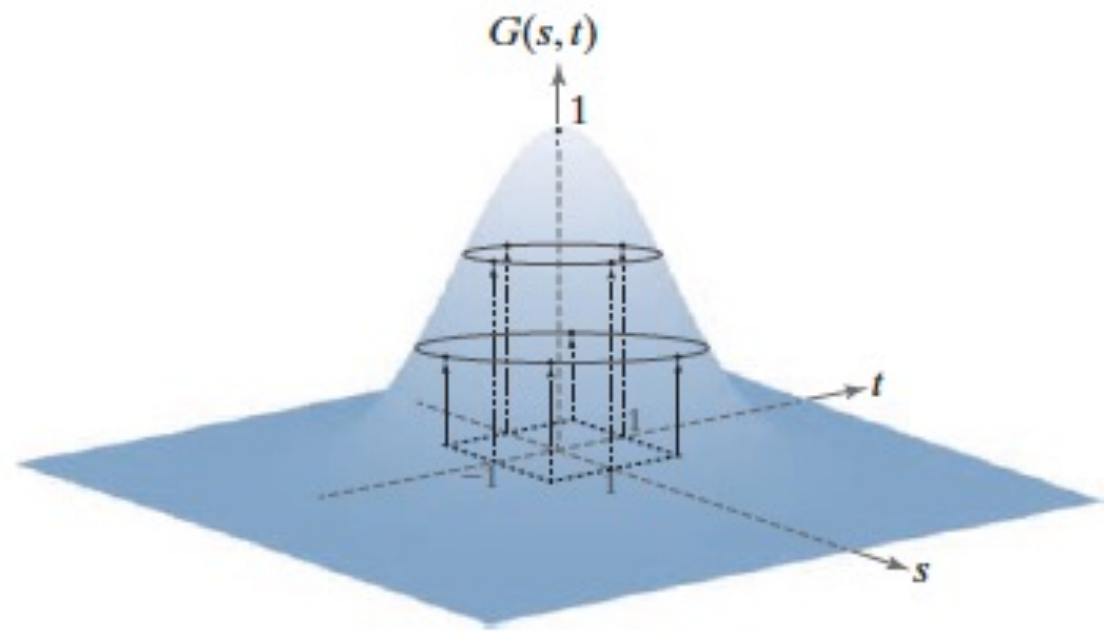
\includegraphics[width=0.7\linewidth]{1.png}

\caption{Image credit: Week3 Lecture2}
\label{fig: gaussian kernel}
\end{figure}

For the sobel mask, depends on the direction of the $x,y$, the matrix $\bf{X}$ can get by the Smoothing and Filtering in $x$.

\begin{equation*}
      \bf{X}=\left(         
  \begin{array}{ccc}  
    -1 & 0 & 1\\  
    -2 & 0 & 2\\  
    -1 & 0 & 1 \\
  \end{array}
\right)  
\end{equation*}
By the same way but in $y$, we have the $\bf{Y}$
\begin{equation*}
      \bf{Y}=\left(         
  \begin{array}{ccc}  
    -1 & -2 & -1\\  
    0 & 0 & 0\\  
    1 & 2 & 1 \\
  \end{array}
\right)  
\end{equation*}



%-------------------------------------------------------------------------
\subsubsection{Non-Maximum Suppression}
Non-Maximum Suppression(NMS) which suppressing elements that are not maxima can be understood as local maximum search. The equation as following
\begin{equation*}\label{eq: nonmaxsup}
M(x,y)= \begin{cases}
|\nabla S|(x,y),  &\text{if } |\nabla S|(x,y) > |\triangle S|(x^\prime,y^\prime)  \& \\ 
&|\triangle S|(x,y)>|\triangle S|(x^{\prime \prime},y^{\prime \prime});    \\
0,  &\text{Otherwise}
\end{cases}
\end{equation*}
where $x ^\prime $ and $x^{\prime \prime} $ are the neighbors of x along normal direction to an edge.

\subsubsection{Hysteresis Thresholding}
In the Hysteresis Thresholding, we have two parameters $H$ and $L$, which mean 'High' and 'Low'. Any gradient at a pixel which above 'High', declare it as an 'edge pixel'. On the contrary, the pixel gradient below 'Low' is the 'non-edge-pixel'. For the between $H$ and $L$, we need consider its neighbors iteratively. 


%------------------------------------------------------------------------
\subsection{Edge Detection using Laplacian of Gaussian}\label{sec: log}
For the Laplacian of Gaussian(LOG), we can consider the The second derivative of Eq. \eqref{eq: gaussian kernel}, and without $K$, it becomes:
\begin{align}
   & \nabla ^2[f(x,y)*G(x,y)]=\nabla ^2 G(x,y)*f(x,y) \\
   & \nabla ^2 G(x,y)= \frac{x^2+y^2-\sigma^2}{\sigma^4} exp\{-\frac{x^2+y^2}{2\sigma^2}\}
\end{align}

\subsection{blob Detection}
The Sec. \ref{sec: log}, shows the LOG, we can find the characteristic scale of the 
blob by convolving it with Laplacian at several scales. But there is an issue that Laplacian response decays as scale increases.

Hence, we need normalization, which is multiply Gaussian derivative by $\sigma$ and multiply Laplacian by $\sigma^2$. The result is shown below:
\begin{figure}[htbp]
\centering

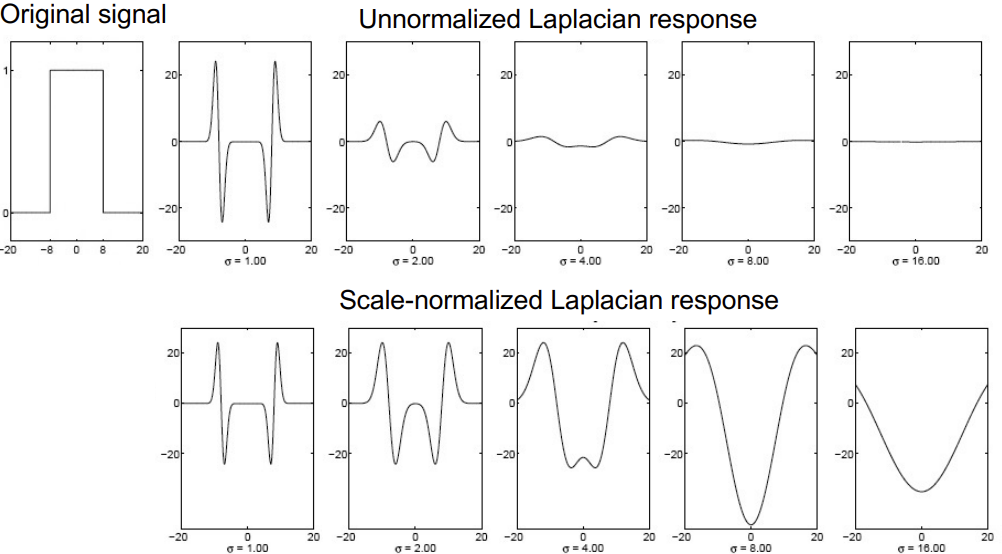
\includegraphics[width=1\linewidth]{2.png}

\caption{Image credit: Week5 Lecture1}

\end{figure}


\section{Results and Analysis}

\subsection{Canny Edge Detection \& Edge Detection using LOG}
The Fig. \ref{fig:canny} shows our result and progress of canny edge detection. Pictures of the process are shown in the Appendix \ref{sec: allcanny}.

\begin{figure}[h]
\centering
\subfigure[]{
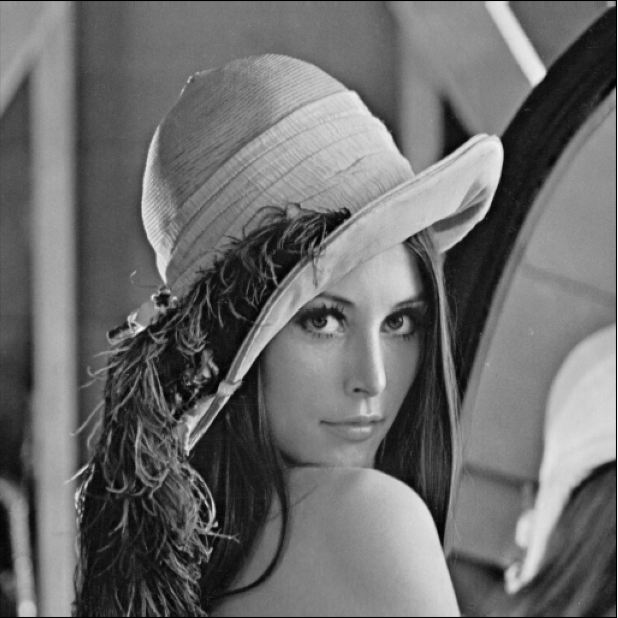
\includegraphics[width=0.4\linewidth]{3.png}
}
\quad
\subfigure[]{
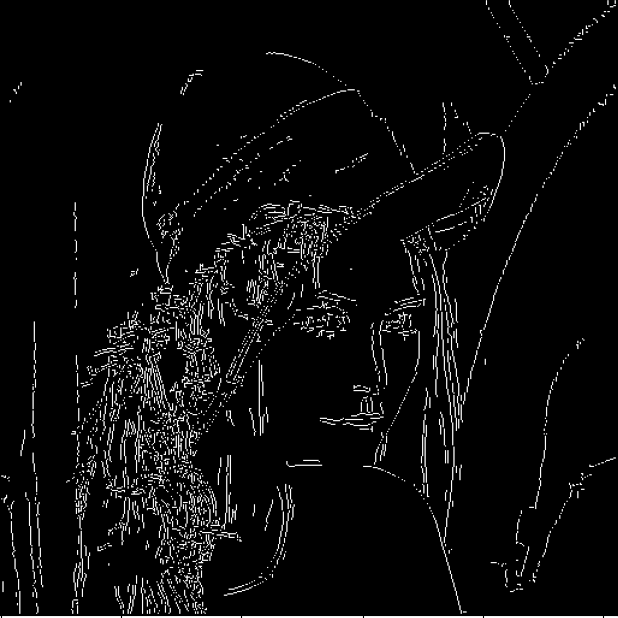
\includegraphics[width=0.4\linewidth]{10.png}
}
\caption{(a) original figure, (b) the Canny Edge Detection}
\label{fig:canny}
\end{figure}
The LoG edge detection's result is shown at Fig \ref{fig: log}


\begin{figure}[htbp]
\centering

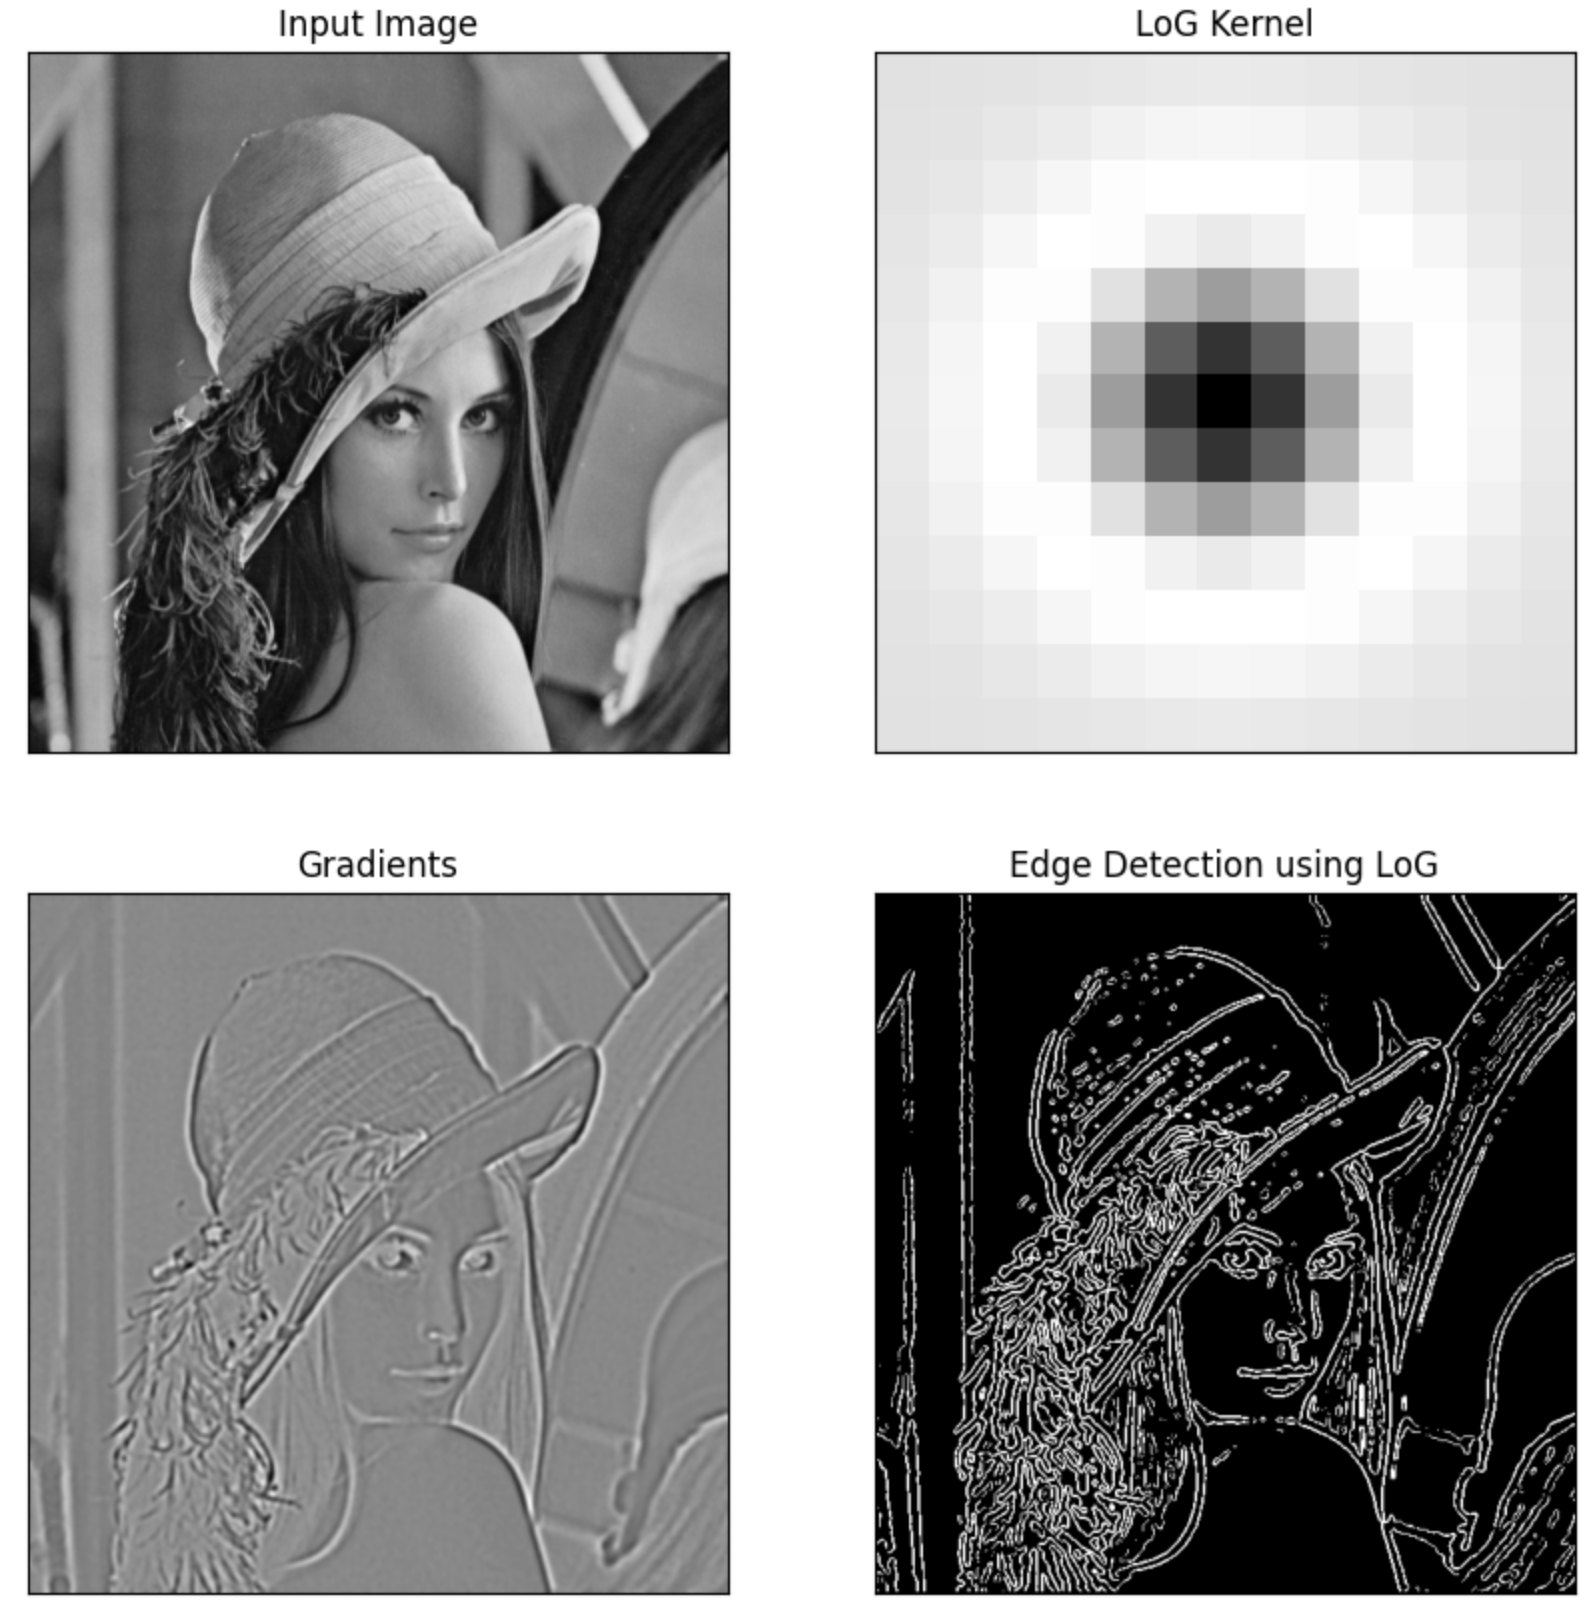
\includegraphics[width=0.7\linewidth]{11.png}

\caption{Edge Detection using LOG}
\label{fig: log}
\end{figure}

By observing Fig. \ref{fig:canny} and Fig. \ref{fig: log} and analyzing the principle of two ways, we can draw the following conclusions:

\begin{enumerate}
\item The LoG operator detects more details than the Canny operator,
\item Canny edge detectors are not susceptible to noise, while LOG operators at the same scale are susceptible to noise,
\item LoG might contain some false edges,
\item LoG will ignore some textural regions.
\end{enumerate}

\subsection{Blob Detection}
Depending on the normalized or without normalized, and different threshold values. We have the Fig. \ref{fig:partblob}, which we only show the best results (See the appendix \ref{sec: allblob} for a full comparison of parameters)

\begin{figure}[h]
\centering
\subfigure[]{
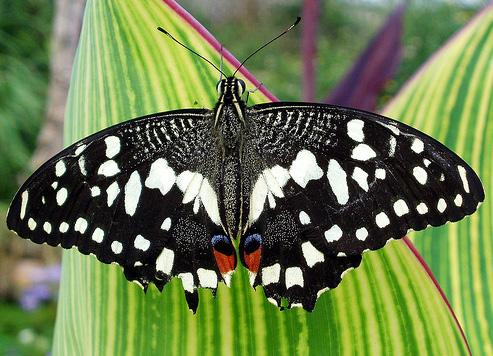
\includegraphics[width=0.4\linewidth]{best/sunflower_unnormalized_squared_t=0.15_s=5.png}
}
\quad
\subfigure[]{
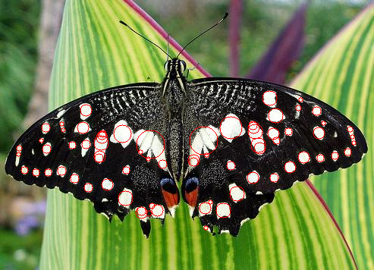
\includegraphics[width=0.4\linewidth]{图片1.png}
}
\quad
\subfigure[]{
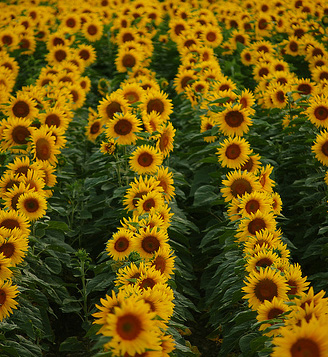
\includegraphics[width=0.4\linewidth]{sunflower_unnormalized_squared_t=0.15_s=5.png}
}
\quad
\subfigure[]{
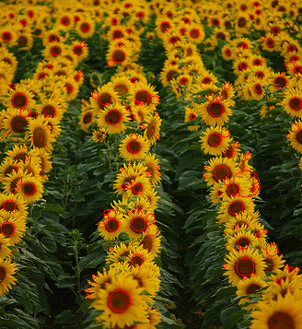
\includegraphics[width=0.4\linewidth]{图片2.png}
}
\caption{(a) original figure, (b) threshold=$0.15$, $s=3/\sqrt{2.5}$, (c) original figure, (d) threshold=$0.04$,$s=2/\sqrt{2.5}$ }
\label{fig:partblob}
\end{figure}

Combine with appendix \ref{sec: allblob}, we know that to ensure that the amplitude obtained by Gaussian filtering is approximately equal at different scales normalized is necessary.  


\clearpage

\onecolumn

\begin{appendices}\label{append}

\section{Edge Detection}\label{sec: allcanny}
\subsection{Canny Edge Detection}
The fig. \ref{fig:cannyall} shows the process of Canny edge detection. We adjust the Low values $[5,10,15,20,25,30,35,40]$ and $High-Low=[20,25,30,35,40,45,50,55]$ which can see in fig. 
\begin{figure}[h]
  \centering
  \subfigure[]{
  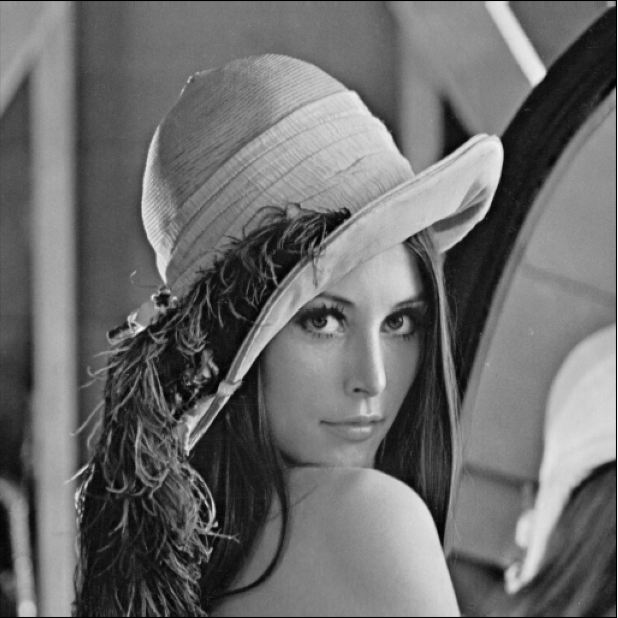
\includegraphics[width=0.2\textwidth]{3.png}
  }
  \quad
  \subfigure[]{
  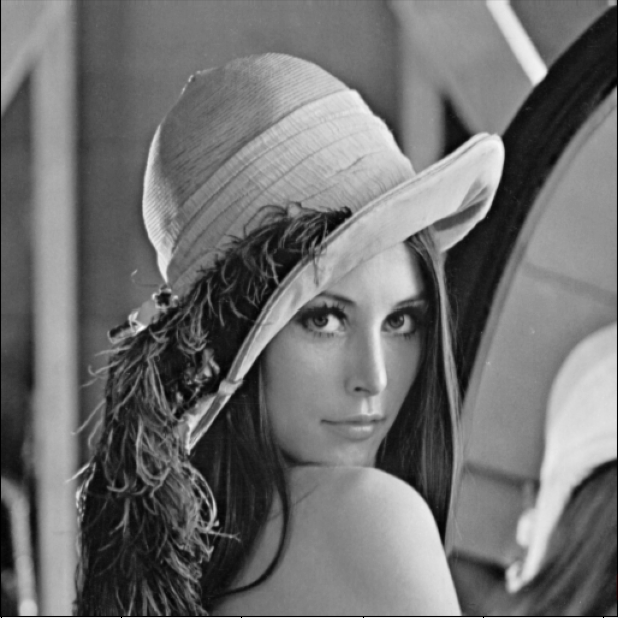
\includegraphics[width=0.2\textwidth]{4.png}
  }
  \quad
  \subfigure[]{
  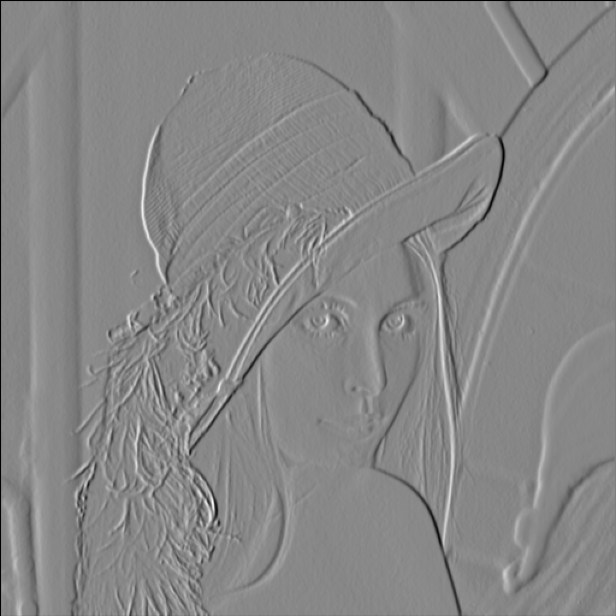
\includegraphics[width=0.2\textwidth]{5.png}
  }
  \quad
  \subfigure[]{
  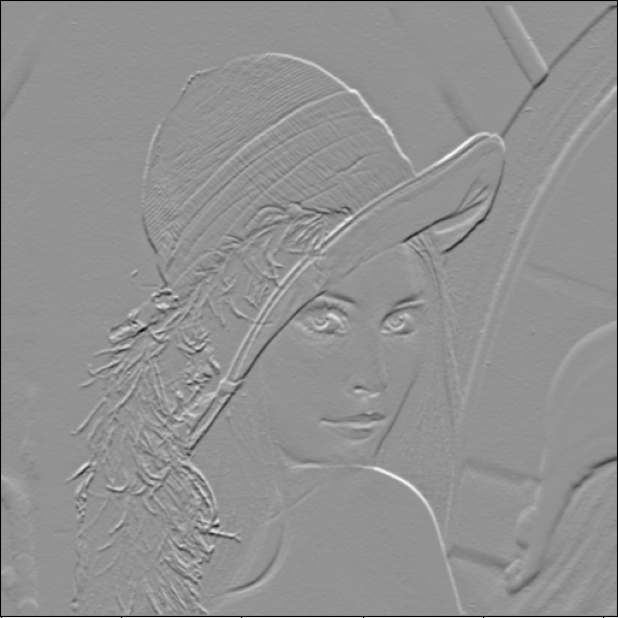
\includegraphics[width=0.2\textwidth]{6.png}
  }
  \quad
  \subfigure[]{
  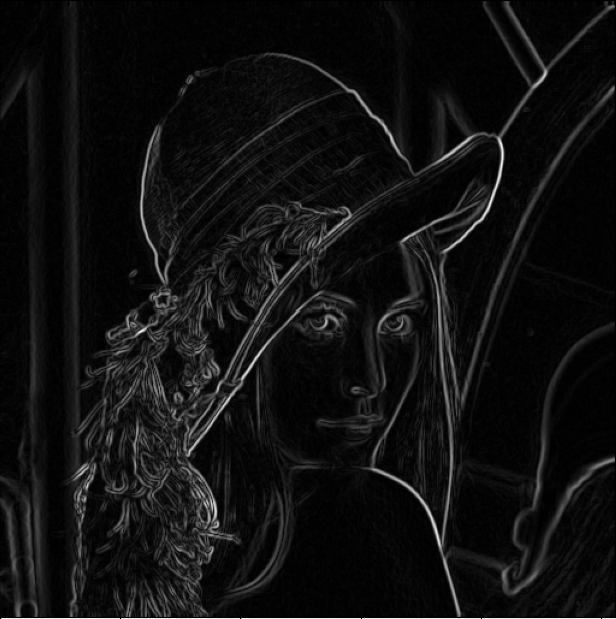
\includegraphics[width=0.2\textwidth]{7.png}
  }
  \quad
  \subfigure[]{
  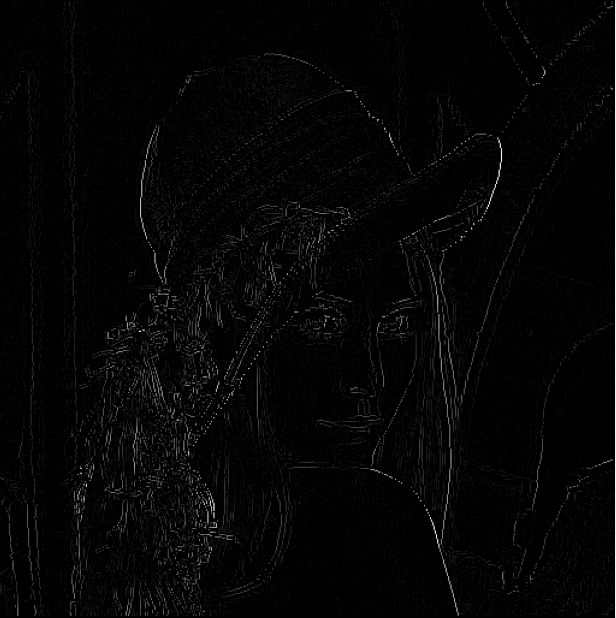
\includegraphics[width=0.2\textwidth]{8.png}
  }
  \quad
  \subfigure[]{
  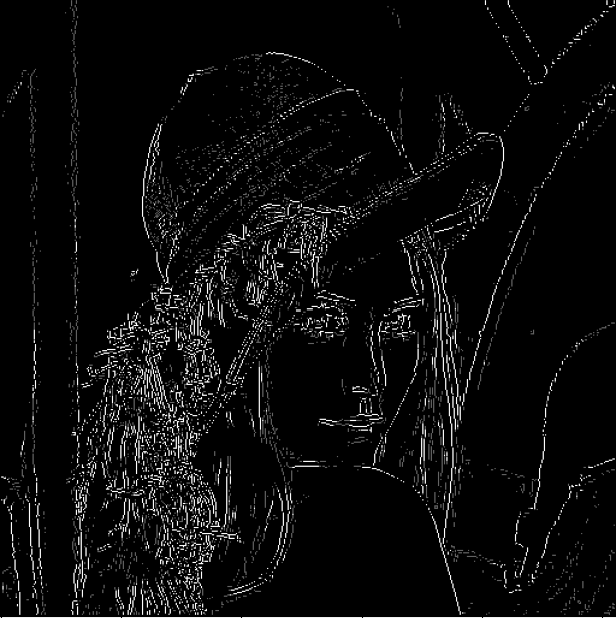
\includegraphics[width=0.2\textwidth]{9.png}
  }
  \quad
  \subfigure[]{
  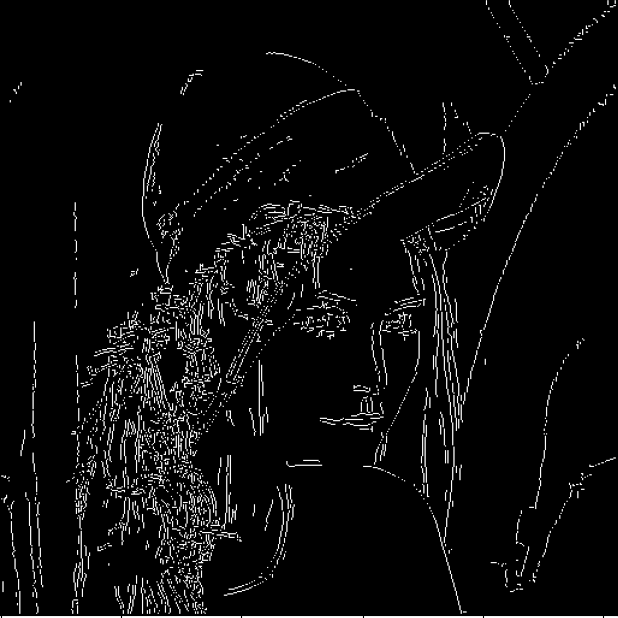
\includegraphics[width=0.2\textwidth]{10.png}
  }
  \caption{(a) original figure, (b) Smoothing, (c) sobel\_x, (d) filter, (e) magnitude of gradients, (f) non-max-suppression, (g) thresholding, (h) hysteresis thresholding}
  \label{fig:cannyall}
  \end{figure}
  
  

  \begin{figure}[hbp]
    \centering
    \subfigure[]{
    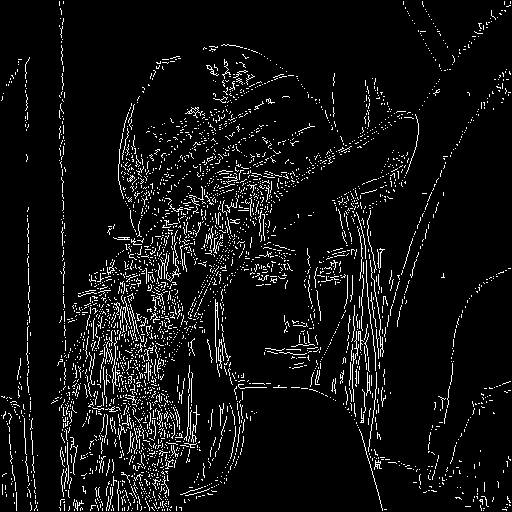
\includegraphics[width=0.2\textwidth]{findbestcanny/Canny_L_H_5_25.png}
    }
    \quad
    \subfigure[]{
    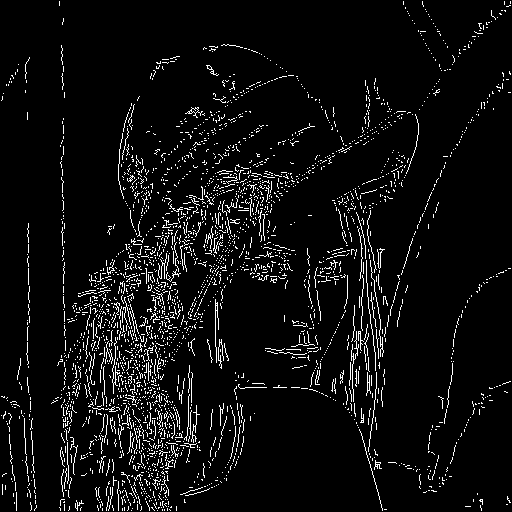
\includegraphics[width=0.2\textwidth]{findbestcanny/Canny_L_H_5_30.png}
    }
    \quad
    \subfigure[]{
    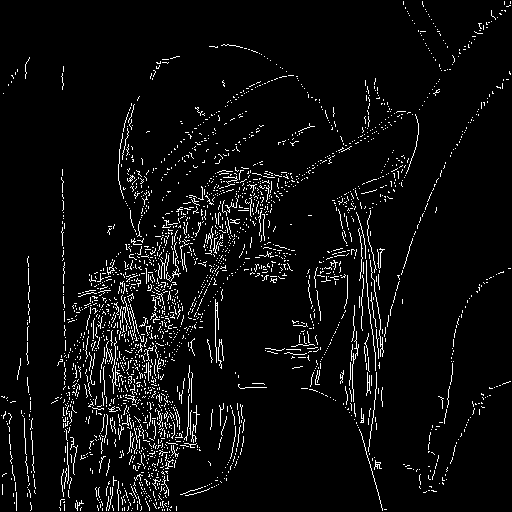
\includegraphics[width=0.2\textwidth]{findbestcanny/Canny_L_H_5_35.png}
    }
    \quad
    \subfigure[]{
    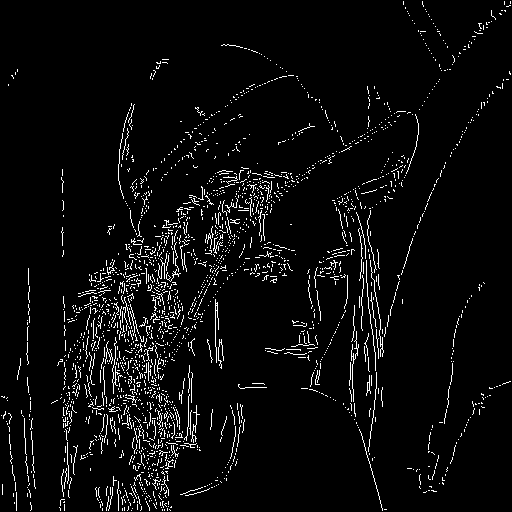
\includegraphics[width=0.2\textwidth]{findbestcanny/Canny_L_H_5_40.png}
    }
    \quad
    \subfigure[]{
    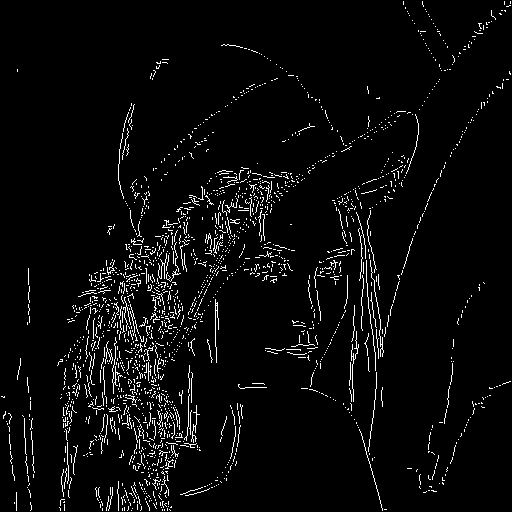
\includegraphics[width=0.2\textwidth]{findbestcanny/Canny_L_H_5_45.png}
    }
    \quad
    \subfigure[]{
    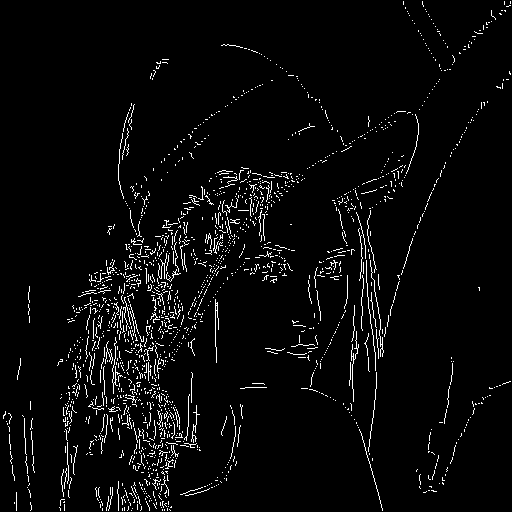
\includegraphics[width=0.2\textwidth]{findbestcanny/Canny_L_H_5_50.png}
    }
    \quad
    \subfigure[]{
    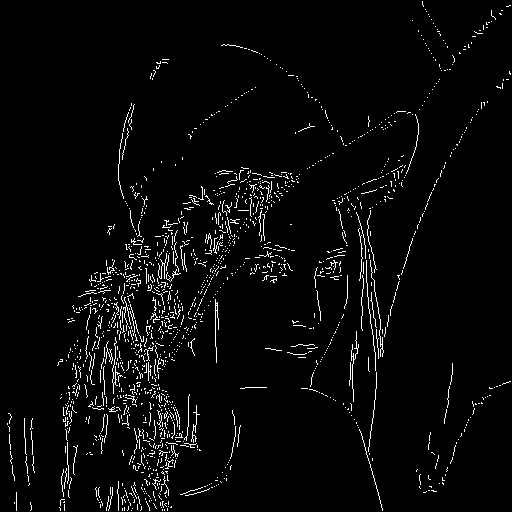
\includegraphics[width=0.2\textwidth]{findbestcanny/Canny_L_H_5_55.png}
    }
    \quad
    \subfigure[]{
    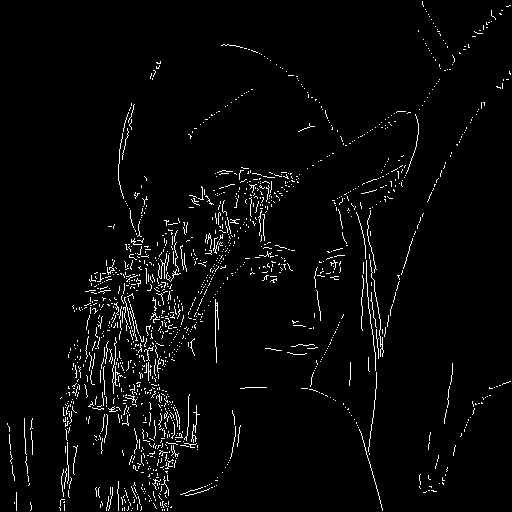
\includegraphics[width=0.2\textwidth]{findbestcanny/Canny_L_H_5_60.png}
    }
    \caption{This is the $Low=5$}
    \label{fig: Low5}
    \end{figure}

    \begin{figure}[htbp]
      \centering
      \subfigure[]{
      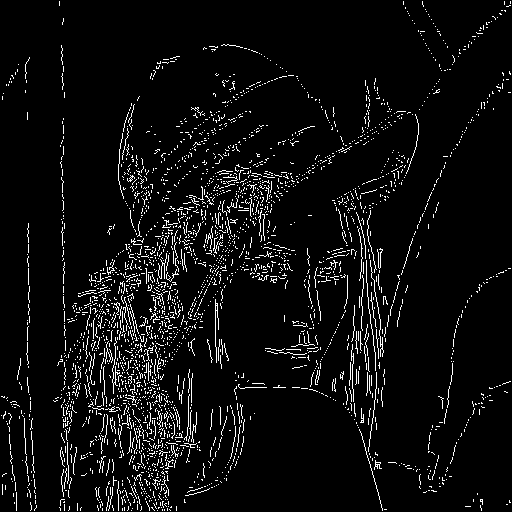
\includegraphics[width=0.2\textwidth]{findbestcanny/Canny_L_H_10_30.png}
      }
      \quad
      \subfigure[]{
      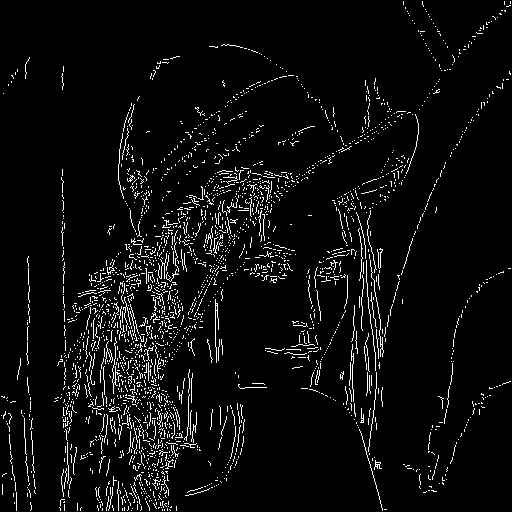
\includegraphics[width=0.2\textwidth]{findbestcanny/Canny_L_H_10_35.png}
      }
      \quad
      \subfigure[]{
      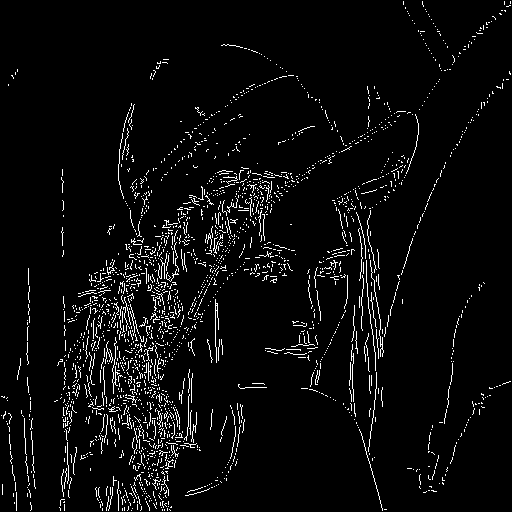
\includegraphics[width=0.2\textwidth]{findbestcanny/Canny_L_H_10_40.png}
      }
      \quad
      \subfigure[]{
      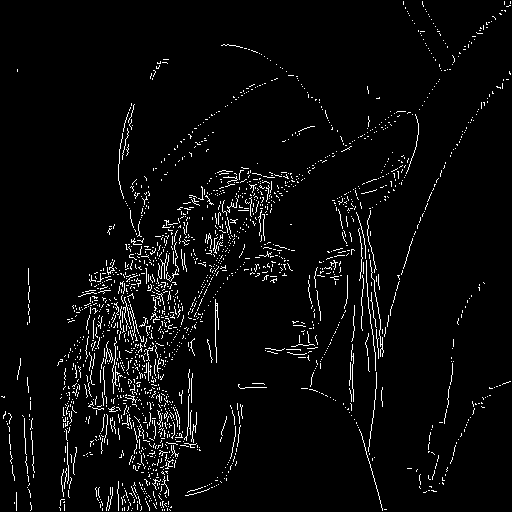
\includegraphics[width=0.2\textwidth]{findbestcanny/Canny_L_H_10_45.png}
      }
      \quad
      \subfigure[]{
      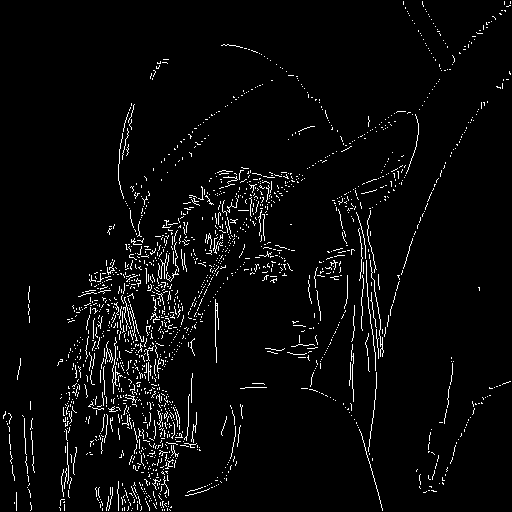
\includegraphics[width=0.2\textwidth]{findbestcanny/Canny_L_H_10_50.png}
      }
      \quad
      \subfigure[]{
      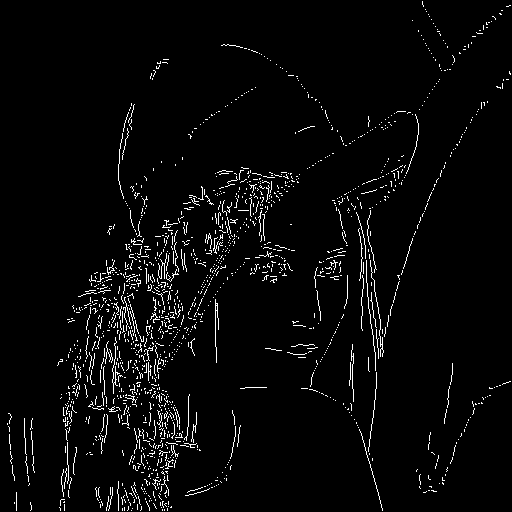
\includegraphics[width=0.2\textwidth]{findbestcanny/Canny_L_H_10_55.png}
      }
      \quad
      \subfigure[]{
      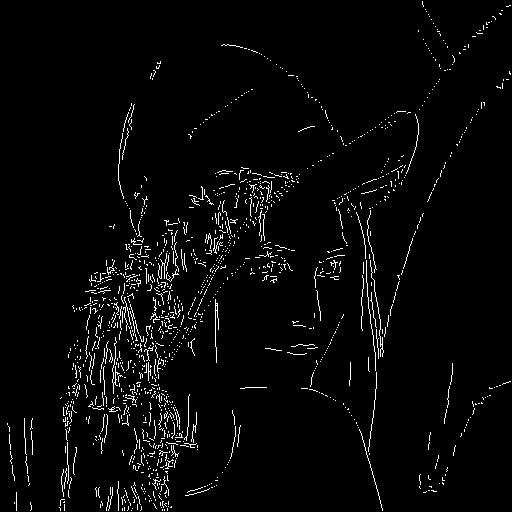
\includegraphics[width=0.2\textwidth]{findbestcanny/Canny_L_H_10_60.png}
      }
      \quad
      \subfigure[]{
      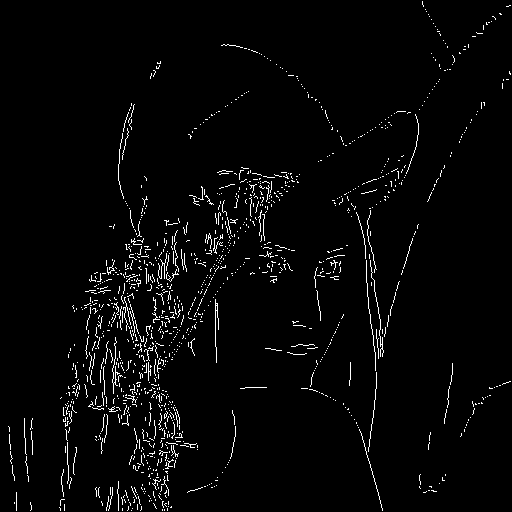
\includegraphics[width=0.2\textwidth]{findbestcanny/Canny_L_H_10_65.png}
      }
      \caption{This is the $Low=10$}
      \label{fig: Low10}
      \end{figure}
\section{Blob Detection}\label{sec: allblob}



\section{Butterfly}





\end{appendices}







\end{document}